\section{Determinantes}
\label{sec:det}
   O determinante é uma função definida de forma bem específica sobre os elementos de uma matriz. Essa função
associa a matriz à um número real. Somente matrizes quadradas possuem determinantes.
   O determinante de uma matriz A se escreve, como det(A) ou como |A|, ou ainda como ||A||.
A definição matemática dessa função é complicada e vou omitir nesse texto. Meu objetivo é mostrar como se calcula
 o determinante de uma matriz. Informações mais específicas podem ser encontradas na referencia 1.
   \subsection{Algumas propriedades}
   \begin{itemize}
\label{prop:det}     
     \item O determinante de uma matriz de ordem 1, é o próprio elemento da matriz.
     \item Uma matriz com uma linha ou coluna inteira composta de 0's possui determinante nulo.
     \item Se uma matriz é triangular (superior ou inferior), então seu determinante será o produto dos elementos da diagonal principal\footnote{Essa propriedade é muito útil para calcular o determinante de uma matriz de ordem maior que 3}.
     \item Se A possui 2 linhas ou colunas iguais, então $det(A)=0$.
     \item Quando se multiplica uma linha (ou coluna) da matriz A por um real $\lambda $, o determinante da matriz resultante é igual a $\lambda \cdot det(A)$.
     \item Ao permutar 2 linhas ou colunas da matriz A, o determinante da matriz resultante vale $-det(A)$.
     \item Somar à uma linha (ou coluna) de A uma linha (ou coluna) de A multiplicada por um real não altera o valor do determinante de A.
     \item Se A possui inversa, então $det(A^{-1})=1/det(A)$.
     \item Se 1 linha ou coluna do determinante for combinação linear das outras, então o determinante é nulo.
   \end{itemize}
   \subsection{Determinantes de matrizes de ordem 2}
   Suponha a matriz: $A=\begin{bmatrix}a & b\\c & d\end{bmatrix}$\\
   Seu determinante é obtido multiplicando os elementos da diagonal principal e subtraindo o resultado do produto dos elementos da diagonal secundaria, ou de forma mais simples:\[ det(A)=
   \begin{vmatrix}a & b\\c & d\end{vmatrix}=a\cdot d-b\cdot c\]
   
   \subsection{Determinantes de matrizes de ordem 3}
  
Seja a matriz $A=\begin{bmatrix}
     a & b & c\\d & e & f\\g & h & i
   \end{bmatrix}$\\
   Seu determinante é: $det(A)=aei+bfg+cdh-afh-bdi-ceg$\\
   \begin{figure}[t]
   \centering
     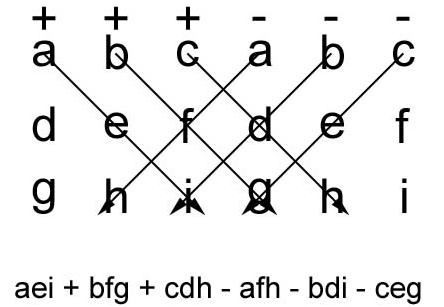
\includegraphics[scale=0.3]{Determinant_3x3-wikipedia.jpg}
     \caption{Regra de Sarrus, note que a repetição da $3^a$ coluna não é necessária. Fonte: Wikipedia, citado nas referencias.}
     \label{fig1}
   \end{figure}
%A figura deve ir antes desse texto por causa do label.
Uma forma prática de calcular esse determinante é a \textit{regra de Sarrus}, na qual se copiam as duas primeiras 
colunas da matriz ao final da mesma e se atribuem os sinais de acordo com a figura~\ref{fig1}
   
   \subsection{Determinantes de ordem maior que 3}
   \subsubsection*{Método de Laplace}
   \addcontentsline{toc}{subsubsection}{Método de Laplace}
   \paragraph*{Cofator} \label{par:cof}O cofator $A_{ij}$ obtido a partir do elemento $a_{ij}$ da matriz A é obtido multiplicando-se o fator $-1^{i+j}$ pelo determinante da matriz A, excluídas a linha i e coluna j. Por exemplo:
\begin{displaymath}
    \text{Seja A=}\begin{bmatrix}
     a & b & c\\d & e & f\\g & h & i
   \end{bmatrix}
\end{displaymath}
   $\text{O cofator }A_{11}=-1^{1+1}\cdot \begin{vmatrix}
     e & f\\h & i
   \end{vmatrix}\quad A_{12}=-1^{1+2}\cdot \begin{vmatrix}
     d & f\\g & i
   \end{vmatrix}$
   
   O método de Laplace consiste em escolher 1 linha (ou coluna) da matriz A e somar os produtos dos elementos da linha (ou coluna) escolhida pelos respectivos cofatores. Usando a matriz $A_{3\times 3}$ definida antes, vamos calcular seu determinante pelo método de Laplace, vou escolher a linha 1 para eliminar:
   \begin{align*}
     det(A)=&a\cdot A_{11}+b\cdot A_{12}+c\cdot A_{13}\\
     &= a\cdot (-1)^2\cdot \begin{vmatrix} e & f\\h & i\end{vmatrix}+b\cdot(-1)^{3}\cdot
      \begin{vmatrix}d & f\\g & i\end{vmatrix}+  c\cdot (-1)^4\cdot \begin{vmatrix}d & e\\g & h\end{vmatrix}
   \end{align*}
   \subsubsection*{Método da triangularização}
	\addcontentsline{toc}{subsubsection}{Método da triangularização}
	
   Este método se baseia na propriedade vista na seção~\ref{prop:det} que diz que o determinante de uma matriz triangular é o produto dos elementos da diagonal principal. Então o trabalho é transformar o determinante da matriz A no determinante de uma matriz triangular usando operações elementares e lembrando que:
   \begin{itemize}
     \item Quando se multiplica uma linha (ou coluna) da matriz A por um real $\lambda $, o determinante da matriz resultante é igual a $\lambda \cdot det(A)$.
     \item Ao permutar 2 linhas ou colunas da matriz A, o determinante da matriz resultante vale $-det(A)$.
     \item Somar à uma linha (ou coluna) de A uma linha (ou coluna) de A multiplicada por um real não altera o valor do determinante de A.
   \end{itemize}
   Um exemplo: Seja A=$\begin{bmatrix}
     1 & 2 &  1 & 2 \\0 &  1 & 2 & 1\\1 &1 &1 &1\\2 & 0& 1 & 3
   \end{bmatrix}$, calcule $det(A)$\\
   Vamos usar o método de Gauss usando os elementos da diagonal principal como pivôs para
 triangularizar este determinante:
   \begin{align*}
    \begin{vmatrix}
      1 & 2 &  1 & 2 \\0 &  1 & 2 & 1\\1 &1 &1 &1\\2 & 0& 1 & 3
    \end{vmatrix}=
    \begin{vmatrix}
      1 & 2 &  1 & 2 \\0 &  1 & 2 & 1\\0 &-1 &0 &-1\\0 & -4& -1 & -1
    \end{vmatrix}=
    \begin{vmatrix}
      1 & 2 &  1 & 2 \\0 &  1 & 2 & 1\\0 &0 &2 &0\\0 & 0& 7 & 3
    \end{vmatrix}=
    \begin{vmatrix}
      1 & 2 &  1 & 2 \\0 &  1 & 2 & 1\\0 &0 &2 &0\\0 & 0& 0 & 3
    \end{vmatrix}=6
   \end{align*}
Neste exemplo sempre somamos o produto de uma linha por um número real à outra linha, e portanto
o valor do determinante não é alterado. Um caso um pouco mais complicado:
Calcular:$ \begin{vmatrix} 0 & 1 & 2 \\ 1 & 4 & 3 \\ 2 & 2 & 2 \end{vmatrix}$\\
Primeiro vou trocar de lugar a $1^a$ com a $2^a$ linhas:
\[\begin{vmatrix} 0 & 1 & 2 \\ 1 & 4 & 3 \\ 2 & 2 & 2 \end{vmatrix} =- \begin{vmatrix}  1 & 4 & 3\\0 & 1 & 2  \\ 2 & 2 & 2 \end{vmatrix}=\]
Agora vou colocar o 2 da $3^a$ linha para fora do determinante:
\[=-2 \begin{vmatrix}  1 & 4 & 3\\0 & 1 & 2  \\ 1 & 1 & 1 \end{vmatrix}= \]
Usando o método de Gauss para triangularizar o determinante, resulta:
\[=-2 \begin{vmatrix}  1 & 4 & 3\\0 & 1 & 2  \\ 0 & 0 & 4 \end{vmatrix}= -2 \cdot 4 = -8\]

   \newpage
   
\section{Referencias Bibliográficas}
\begin{enumerate}
  \item Álgebra Linear e Aplicações; Callioli,A. C., Domingues, H. H., Costa, R. C. F., $6^{\underline{a}}$ edição.
  \item http://pt.wikipedia.org/wiki/Determinante
  \item http://mathworld.wolfram.com/MatrixInverse.html - artigo sobre matrizes inversas, em inglês.
\end{enumerate}
